\documentclass[bigger]{beamer}
\usepackage[utf8]{inputenc}

%\usepackage{emerald}
\usepackage[T1]{fontenc}
\usepackage[absolute,overlay]{textpos}
%\usepackage[bookmarks=false,pdffitwindow]{hyperref}
%\usepackage{fancybox}
\usepackage{tikz}
\usepackage{graphicx}
\usepackage{minted}
\usepackage{multimedia}
\usepackage{animate}
\usepackage{xcolor}
\usepackage{calc}

\usetheme{CambridgeUS}
\definecolor{RawSienna}{cmyk}{0,0.72,1,0.45}
\usecolortheme[named=RawSienna]{structure}
\usetikzlibrary{shapes.geometric, arrows}

% flowchart settings

\tikzstyle{every node}=[font=\small]
\tikzstyle{block} = [rectangle, draw, fill=blue!20, text centered, text width=12em, rounded corners, node distance=1.3cm]
\tikzstyle{line} = [draw, -latex']


%
% Boxed environment with semi-transparent shadow.
%
\newlength{\boxw}
\newlength{\boxh}
\newlength{\shadowsize}
\newlength{\boxroundness}
\newlength{\tmpa}
\newsavebox{\shadowblockbox}

\setlength{\shadowsize}{6pt}
\setlength{\boxroundness}{3pt}

\newenvironment{shadowblock}[1]%
{\begin{lrbox}{\shadowblockbox}\begin{minipage}{#1}}%
{\end{minipage}\end{lrbox}%
\settowidth{\boxw}{\usebox{\shadowblockbox}}%
\settodepth{\tmpa}{\usebox{\shadowblockbox}}%
\settoheight{\boxh}{\usebox{\shadowblockbox}}%
\addtolength{\boxh}{\tmpa}%

\begin{tikzpicture}
\addtolength{\boxw}{\boxroundness * 2}
\addtolength{\boxh}{\boxroundness * 2}

\foreach \x in {0,.05,...,1}
{
\setlength{\tmpa}{\shadowsize * \real{\x}}
\fill[xshift=\shadowsize - 1pt,yshift=-\shadowsize + 
1pt,black,opacity=.04,rounded corners=\boxroundness] 
(\tmpa, \tmpa) rectangle +(\boxw - \tmpa - \tmpa, \boxh - \tmpa - 
\tmpa);
}

\filldraw[fill=yellow!50, draw=black!50, rounded corners=\boxroundness] (0, 
0) rectangle (\boxw, \boxh);
\draw node[xshift=\boxroundness,yshift=\boxroundness,inner sep=0pt,outer 
sep=0pt,anchor=south west] (0,0) {\usebox{\shadowblockbox}};
\end{tikzpicture}}


\begin{document}
\logo{  \includegraphics[scale=0.06,keepaspectratio]{Imagenes/logos.png}}
\title{3D sensors and Python:\\ A space odyssey \\[0.5cm]}
\subtitle{Celia Cintas \\[0.2cm] EuroPython 2014 \\[0.3cm]
\includegraphics[scale=0.2]{Imagenes/hall360.png}}
\date{}
\begin{frame}
\titlepage
\end{frame}
\section{Introduction}
%\begin{frame}[fragile]{ The Speaker}
%	\texttt{\$ whoami}
%		\begin{itemize}
%			\item 
%		\end{itemize}
%\end{frame}
\begin{frame}{\$ whoami}
\begin{itemize}
    \item PhD Student in Computer Science.
    \item Assistant Professor at UNPSJB.
    \item Work in CENPAT-CONICET and Imaging Science Lab.
    \item Co-Organizer of SciPyCon Argentina.
\end{itemize}
\begin{figure}
        \includegraphics[scale = 0.25]{Imagenes/uni.png}
\end{figure}
\end{frame}

\begin{frame}[t]{ HAL 9000 Jr. - The Hardware}
\begin{figure}
		\includegraphics[scale = 0.3]{Imagenes/3dsensors.png}
\end{figure}
\begin{figure}
		\includegraphics[scale = 0.4]{Imagenes/component.png}
\end{figure}
\end{frame}

\section{A tale of OpenNI}
\begin{frame}[fragile]{ What is OpenNI Framework - NITE ??}
\begin{center}
\animategraphics[autoplay,loop, height=5cm]{10}{Imagenes/gif/my_pngfiles_}{0}{37} 
\url{http://structure.io/openni}
\end{center}
\end{frame}

\begin{frame}{ Where can I run it ...??}
\begin{minipage}{0.47\textwidth}
\begin{itemize}
	\item Linux (x86, x64, ARM)
	\item Mac OS X (x64 Intel Processors)
	\item Windows (x86, x64)
%	\item Android
\end{itemize}
\end{minipage}
\begin{minipage}{0.5\textwidth}
\begin{figure}[h]
		\includegraphics[scale = 0.25]{Imagenes/platforms.png}
\end{figure}
\end{minipage}
\end{frame}

%\begin{frame}{ What can I do with it?}
%\begin{figure}[h]
		%\includegraphics[scale = 0.22]{Imagenes/what.png}
%\end{figure}
%\end{frame}

\begin{frame}{ What can I do with it?}

\begin{figure}[h]
		\includegraphics[scale = 0.22]{Imagenes/what_2.png}
\end{figure}
\tiny{Images from Smart Terrain \texttrademark of Vuforia\texttrademark, xbmc, ninja-fruit, Ni-Mate, Artec Studio\\ and QBo Robot}
\end{frame}

\begin{frame}[fragile]{ Python bindings}
\begin{itemize}
	\item PyOpenNI\\
    (\url{https://github.com/jmendeth/PyOpenNI})
	\item primesense \\ 
    \url{https://pypi.python.org/pypi/primesense/2.2.0.30-3})
\end{itemize}

\end{frame}
%\begin{frame}[fragile]{Demos}
%\movie[height=5cm,width=10cm]{}{Videos/new.avi}
%\end{frame}
\section{Starting with PyOpenNI}
\begin{frame}[fragile]{ Context and Generators}
\begin{minipage}{0.45\textwidth}
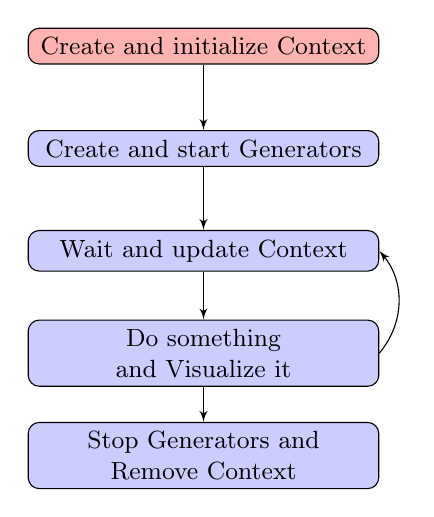
\begin{tikzpicture}
    % Place nodes
    \node [block, fill=red!30] (init) {Create and initialize Context};
    \node [block, below of=init] (generators) {Create and start Generators};
    \node [block, below of=generators] (wait) {Wait and update Context};
    \node [block, below of=wait] (do) {Do something and Visualize it};
    \node [block, below of=do] (stop) {Stop Generators and Remove Context};
    % Draw edges
    \path [line] (init) -- (generators);
    \path [line] (generators) -- (wait);
    \path [line] (wait) -- (do);
    \path [line] (do) -- (stop);
    %\path [line] (viz) -| (wait);
     \path [line] (do.east) to[out=50,in=-50] (wait.east);
\end{tikzpicture}
\end{minipage}
\begin{minipage}{0.5\textwidth}
Different ways to work whith a context:\\
\begin{small}
\begin{minted}{python}
ctx.init()

ctx.init_from_xml_file('conf.xml')

ctx.find_existing_node(type_node)

ctx.open_file_recording('rec.oni')
\end{minted}
\end{small}
\end{minipage}

%\begin{textblock}{4}(2,5.2)
%\begin{shadowblock}{4cm}
%And a small one on top of it.
%\end{shadowblock}
%\end{textblock}

\end{frame}

\begin{frame}{ Context and Generators}
\begin{minipage}{0.45\textwidth}
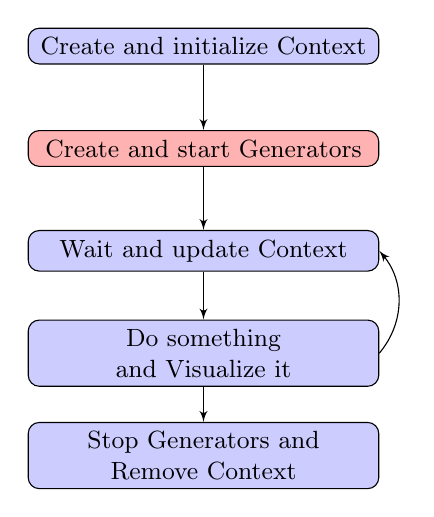
\begin{tikzpicture}
    % Place nodes
    \node [block] (init) {Create and initialize Context};
    \node [block, below of=init, fill=red!30] (generators) {Create and start Generators};
    \node [block, below of=generators] (wait) {Wait and update Context};
    \node [block, below of=wait] (do) {Do something and Visualize it};
    \node [block, below of=do] (stop) {Stop Generators and Remove Context};
    % Draw edges
    \path [line] (init) -- (generators);
    \path [line] (generators) -- (wait);
    \path [line] (wait) -- (do);
    \path [line] (do) -- (stop);
    %\path [line] (viz) -| (wait);
     \path [line] (do.east) to[out=50,in=-50] (wait.east);
\end{tikzpicture}
\end{minipage}
\begin{minipage}{0.45\textwidth}
\begin{itemize}
	\item Image, Depth, IR Generator
	\item User, Gesture, Hand Generator
	\item User Generator has pose and skeleton Capabilities
	\item Register Callbacks to do specific task
	\item Start / Stop wich Generator
	\item Set up fps, resolution, etc.
\end{itemize}
\end{minipage}
\end{frame}

\begin{frame}[fragile]{ Context and Generators}
\begin{minipage}{0.45\textwidth}
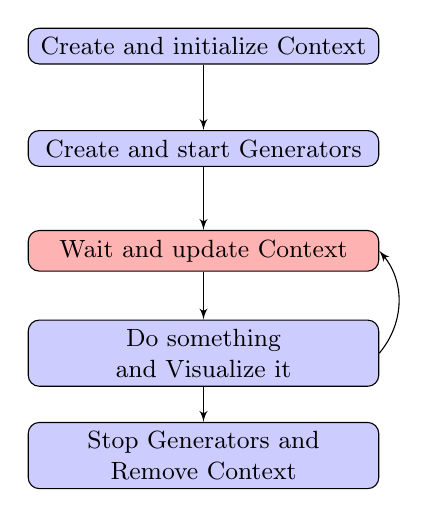
\begin{tikzpicture}
    % Place nodes
    \node [block] (init) {Create and initialize Context};
    \node [block, below of=init] (generators) {Create and start Generators};
    \node [block, below of=generators, fill=red!30] (wait) {Wait and update Context};
    \node [block, below of=wait] (do) {Do something and Visualize it};
    \node [block, below of=do] (stop) {Stop Generators and Remove Context};
    % Draw edges
    \path [line] (init) -- (generators);
    \path [line] (generators) -- (wait);
    \path [line] (wait) -- (do);
    \path [line] (do) -- (stop);
    %\path [line] (viz) -| (wait);
     \path [line] (do.east) to[out=50,in=-50] (wait.east);
\end{tikzpicture}
\end{minipage}
\begin{minipage}{0.5\textwidth}
You can choose when you want to get new data:\\
\begin{minted}{python}
 ctx.wait_and_update_all()

 ctx.wait_none_update_all() 

 ctx.wait_any_update_all()

 ctx.wait_one_update_all(node) 
\end{minted}
%\begin{itemize}
%	\item Wait for X node
%	\item Wait for any node
%	\item Wait for all nodes 
%	\item Or for none ..
%\end{itemize}
\end{minipage}
\end{frame}

\begin{frame}[fragile]{ Context and Generators}
\begin{minipage}{0.45\textwidth}
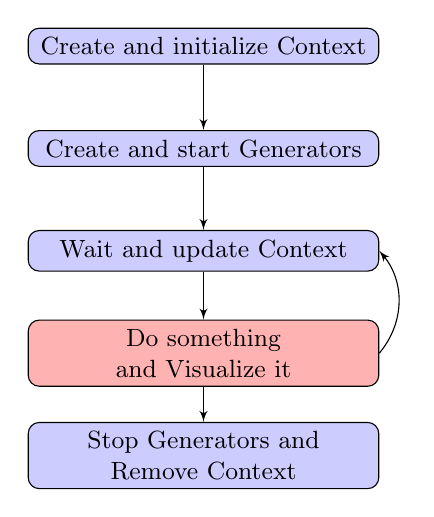
\begin{tikzpicture}
    % Place nodes
    \node [block] (init) {Create and initialize Context};
    \node [block, below of=init] (generators) {Create and start Generators};
    \node [block, below of=generators] (wait) {Wait and update Context};
    \node [block, below of=wait, fill=red!30] (do) {Do something and Visualize it};
    \node [block, below of=do] (stop) {Stop Generators and Remove Context};
    % Draw edges
    \path [line] (init) -- (generators);
    \path [line] (generators) -- (wait);
    \path [line] (wait) -- (do);
    \path [line] (do) -- (stop);
    %\path [line] (viz) -| (wait);
     \path [line] (do.east) to[out=50,in=-50] (wait.east);
\end{tikzpicture}
\end{minipage}
\begin{minipage}{0.5\textwidth}
Some things that you can do:
\begin{small}
\begin{minted}{python}
depth_gen.get_tuple_depth_map()

skel.get_joint_position(id, i)

image_gen.get_raw_image_map_bgr()
\end{minted}
\end{small}
\end{minipage}
\end{frame}

\begin{frame}[fragile]{ Context and Generators}
\begin{minipage}{0.45\textwidth}
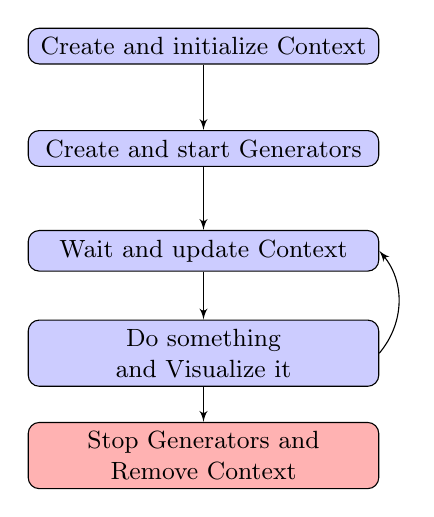
\begin{tikzpicture}
    % Place nodes
    \node [block] (init) {Create and initialize Context};
    \node [block, below of=init] (generators) {Create and start Generators};
    \node [block, below of=generators] (wait) {Wait and update Context};
    \node [block, below of=wait] (do) {Do something and Visualize it};
    \node [block, below of=do, fill=red!30] (stop) {Stop Generators and Remove Context};
    % Draw edges
    \path [line] (init) -- (generators);
    \path [line] (generators) -- (wait);
    \path [line] (wait) -- (do);
    \path [line] (do) -- (stop);
    %\path [line] (viz) -| (wait);
     \path [line] (do.east) to[out=50,in=-50] (wait.east);
\end{tikzpicture}
\end{minipage}
\begin{minipage}{0.5\textwidth}
Ways to stop data acquisition:
\begin{minted}{python}
 ctx.stop_generating_all()

 node_gen.stop_generating()

 ctx.shutdown()
 \end{minted}
\end{minipage}
\end{frame}

\begin{frame}{ Demo Time}
\begin{figure}[h]
		\includegraphics[scale = 0.15]{Imagenes/demo.png}
\end{figure}
\end{frame}


\begin{frame}{ Skeleton Basics}
\begin{minipage}{0.45\textwidth}
Skeleton and Pose Capabilities
\begin{itemize}
	\item Profile
	\item Joints
	\item Start/ Stop Calibration
	\item Start/ Stop Tracking
\end{itemize}
\end{minipage}
\begin{minipage}{0.45\textwidth}
\begin{figure}[h]
		\includegraphics[scale = 0.05]{Imagenes/skeleton.jpg}
\end{figure}
\end{minipage}

\end{frame}

\begin{frame}{ Demo Time}
\begin{figure}[h]
		\includegraphics[scale = 0.15]{Imagenes/demo.png}
\end{figure}
\end{frame}

\begin{frame}{ Hand and Gesture tracking}
\begin{minipage}{0.45\textwidth}
Gesture and Hands Generator
\begin{itemize}
	\item Add/Remove Gestures (Wave, click, etc)
	\item Start/ Stop Tracking
\end{itemize}
\end{minipage}
\begin{minipage}{0.45\textwidth}
\begin{figure}[h]
		\includegraphics[scale = 0.2]{Imagenes/thing.jpg}
\end{figure}
\end{minipage}
\end{frame}

\begin{frame}{ Demo Time}
\begin{figure}[h]
		\includegraphics[scale = 0.15]{Imagenes/demo.png}
\end{figure}
\end{frame}

%\begin{frame}[fragile]{Demos (Cont.)}
%\movie[height=5cm,width=10cm]{}{Videos/popeye.avi}
%\end{frame}

\section{Final Demo}
\begin{frame}{ For the final demo ...}
\begin{figure}[h]
        \includegraphics[scale = 0.35]{Imagenes/final_pochi.png}
\end{figure}
\end{frame}

%\begin{frame}{ PyOpenNI Stuff}

%\end{frame}
\section{Sorry Dave ..}

\begin{frame}{ Q\&A}
\begin{center}
\begin{huge}
Thank you!
\end{huge}
\end{center}
\begin{figure}[h]
		\includegraphics[scale = 0.15]{Imagenes/final.jpg}
\end{figure}
\begin{Small}
\begin{itemize}
    \item \url{https://github.com/celiacintas/3dsensors_talk}
    \item \url{https://github.com/jmendeth/PyOpenNI}
    \item \url{http://structure.io/openni}
\end{itemize}
\end{Small}
\end{frame}

\end{document}